\begin{frame}{Agenda}
\begin{itemize}
    \item Introduction
    \item \textbf{Literature Review}
    \item Methodology
    \item Results
    \item Conclusion and Future Work
\end{itemize}
\end{frame}

%%

\begin{frame}{Literature Review} \pause
    Recommender Systems\\ \pause
    \vspace{0.5cm}
    Clustering\\ \pause
    \vspace{0.5cm}
    Principal Component Analysis (PCA)
\end{frame}

%%

\begin{frame}{Recommender Systems}
    \onslide<2->{Collaborative filtering \\}
    \begin{itemize}
        \item \onslide<5->{user-based} \onslide<6->{- "people like you, also like X"}
        \item \onslide<7->{item-based} \onslide<8->{- "if you like X you may like Y"}
    \end{itemize}
    \onslide<3->{Content-based filtering \\}
        \begin{itemize}
            \item \onslide<9->{user profile}
        \end{itemize}
    \vspace{0.5cm}
    \onslide<4->{Hybrid}
        \begin{itemize}
            \item \onslide<10->{cold start}
            \item \onslide<11->{sparse matrix (data)}
        \end{itemize}
\end{frame}

%%

\begin{frame}{Recommender Systems}
    \begin{figure}
       \centering
       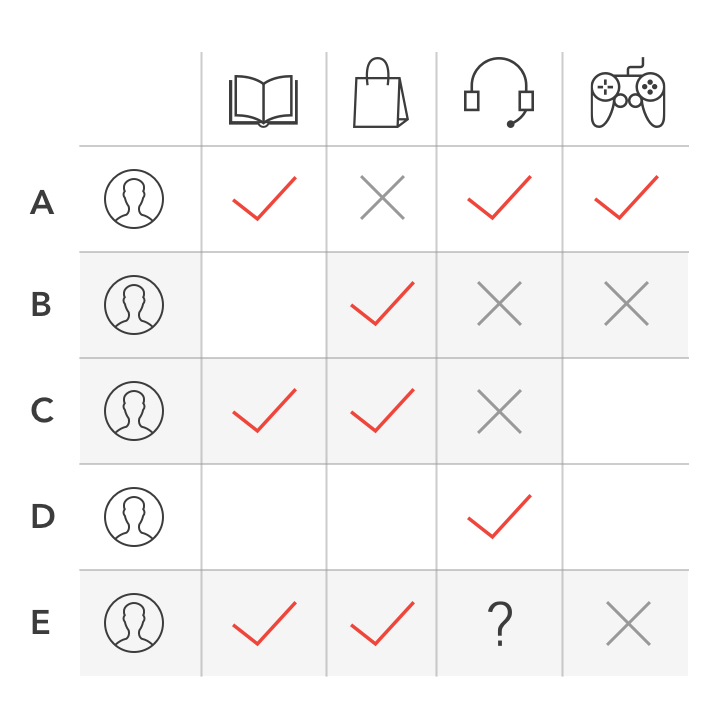
\includegraphics[width=7cm]{fig/ch2-colab-filt-user-user.jpg}
       \caption{User-based logic on collaborative filtering}
    \end{figure}
\end{frame}

%%

\begin{frame}{Recommender Systems - Benefits to business} \pause
    $75\%$ of what people watch on Netflix come from recommendations \\ \pause
    \vspace{0.5cm}
    $70\%$ of people's time spent on YouTube comes from the recommendation \\ \pause
    \vspace{0.5cm}
    $35\%$ of the purchases on Amazon come from recommendations \\ \pause
    \vspace{0.5cm}
    Netflix prize!
\end{frame}

%%

\begin{frame}{Recommender Systems - Lift} \pause
    \begin{column}{.5\textwidth}
        Market: $\mathcal M$ with size $|\mathcal M |\!=\!N$ \\ \pause
        \vspace{0.25cm}
        Leads: $\mathcal L \supset \mathcal M $, with $|\mathcal L|\!=\!n$ \\ \pause
        \vspace{0.25cm}
        $\mathcal L$ is unknown! \\ \pause
    \end{column}
    \begin{column}{.5\textwidth}
        Random chance: $n/N$ \\ \pause
        \vspace{0.25cm}
        Company $X_i$ -> score $S_i$ \\ \pause
        \vspace{0.25cm}
        Ordered: $S_i>S_{i-1}$ from $S_N$ to $S_1$ \\ \pause
    \end{column}
    \vfill
    \begin{column}{\textwidth}
        Given a $k$: \pause
        \vspace{0.25cm}
        \LARGE{
            \begin{equation*}
                \mathrm{lift}_k = \frac{P(X_{i:k\leq i\leq N}\in \mathcal L)}{n/N}
            \end{equation*}
        }
    \end{column}
\end{frame}

%%

\begin{frame}{Recommender Systems - Lift} \pause
    \begin{figure}
        \caption{Rectangular box with colored balls.} \pause
        \begin{subfigure}{\linewidth}
            \centering
            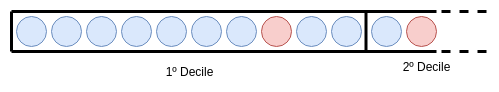
\includegraphics[width=\linewidth]{fig/ch2-rec-box-upper.png}
            \caption{Upper view.}
        \end{subfigure}
        \begin{subfigure}{\linewidth}
            \centering
            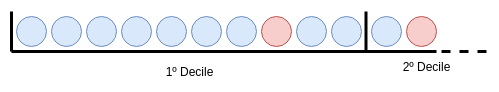
\includegraphics[width=\linewidth]{fig/ch2-rec-box-front.png}
            \caption{Front view.}
        \end{subfigure}
    \end{figure}
\end{frame}

%%

\begin{frame}{Recommender Systems - Lift}
    \begin{figure}
        \caption{Reordering of the balls.} \pause
        \begin{subfigure}{\linewidth}
            \centering
            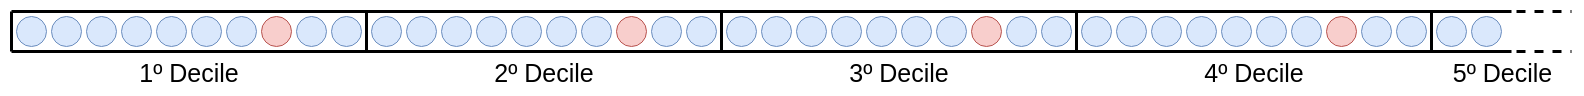
\includegraphics[width=\linewidth]{fig/ch2-rec-box-ordering-before.png}
            \caption{Before.} \pause
        \end{subfigure}
        \begin{subfigure}{\linewidth}
            \centering
            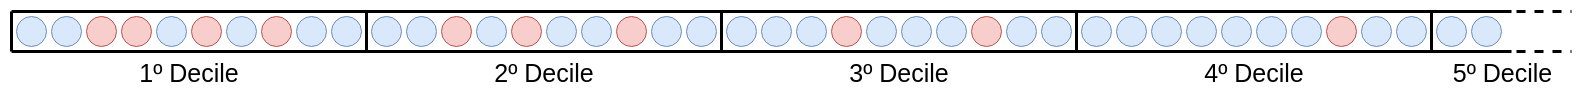
\includegraphics[width=\linewidth]{fig/ch2-rec-box-ordering-after.png}
            \caption{After.}
        \end{subfigure}
    \end{figure}
\end{frame}

%%

\begin{frame}{Recommender Systems - Lift}
    \begin{figure}
       \centering
       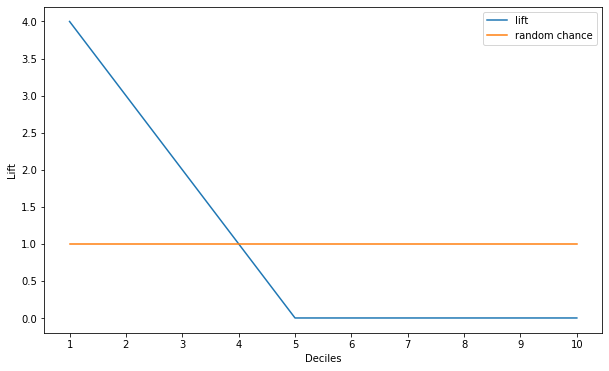
\includegraphics[width=\linewidth]{fig/ch2-lift-plot.png}
       \caption{Lift plot for the reordered box with the random chance.}
    \end{figure}
\end{frame}

%%

\begin{frame}{Clustering} \pause
    Unsupervised learning technique \\ \pause
    \vspace{0.2cm}
    Hidden" structures/patterns in a dataset \\ \pause
    \vspace{0.2cm}
    Several applications \\ \pause
    \begin{itemize}
        \item Engineering and Computer Science \pause
        \item Biology \pause
        \item Astronomy \pause
        \item and more. \pause
    \end{itemize}
    Various approaches \pause
    \begin{itemize}
        \item Connectivity-based \pause
        \item Hierarchical Clustering \pause
        \item Centroid-based \pause
        \item Distribution-based \pause
        \item Density-based
    \end{itemize}
\end{frame}

%%

\begin{frame}{PCA}
    Orthogonal linear transformation \\ \pause
    \vspace{0.5cm}
    Principal Components \pause -> original data variance \\ \pause
    \vspace{0.5cm}
    Uses \pause
    \begin{itemize}
        \item PCA plot \pause
        \item dimensionality reduction
    \end{itemize}
\end{frame}

%

\begin{frame}{PCA}
    \begin{figure}
        \centering
        \caption{PCA algorithm steps.} \pause
        \begin{subfigure}{0.3\textwidth}
            \centering
            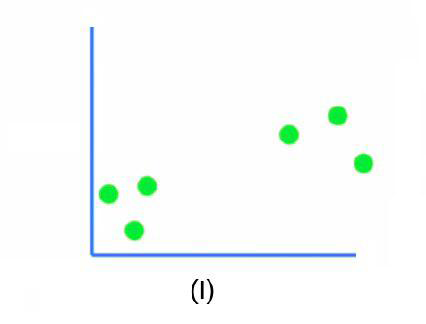
\includegraphics[width=\linewidth]{fig/ch2-pca-steps-01.png}
        \end{subfigure}  \pause
        \begin{subfigure}{0.3\textwidth}
            \centering
            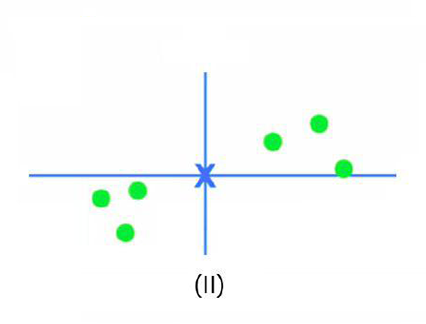
\includegraphics[width=\linewidth]{fig/ch2-pca-steps-02.png}
        \end{subfigure} \pause
        \begin{subfigure}{0.3\textwidth} 
            \centering
            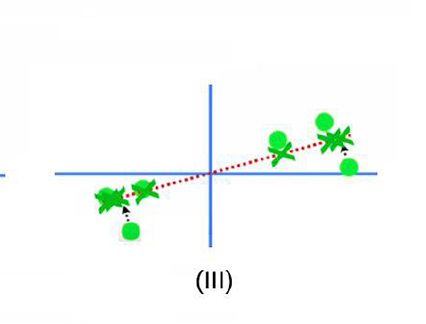
\includegraphics[width=\linewidth]{fig/ch2-pca-steps-03.png}
        \end{subfigure}\vskip 0.3em \pause
        %%
        \begin{subfigure}{0.3\textwidth}
            \centering
            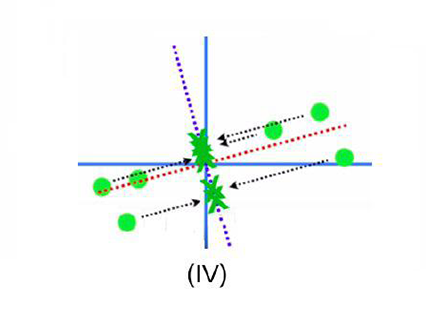
\includegraphics[width=\linewidth]{fig/ch2-pca-steps-04.png}
        \end{subfigure} \pause
        \begin{subfigure}{0.3\textwidth}
            \centering
            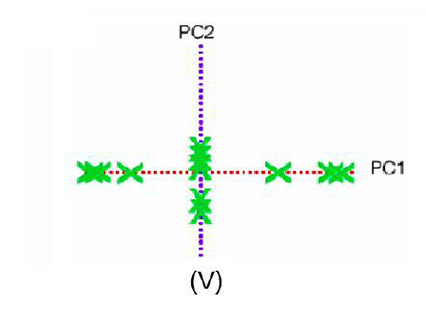
\includegraphics[width=\linewidth]{fig/ch2-pca-steps-05.png}
        \end{subfigure} \pause
        \begin{subfigure}{0.3\textwidth}
            \centering
            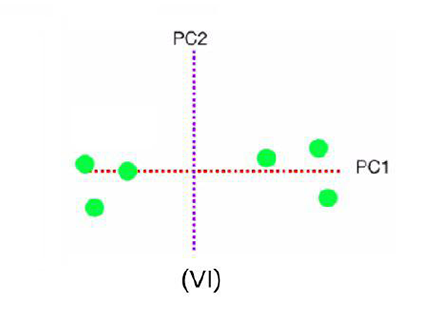
\includegraphics[width=\linewidth]{fig/ch2-pca-steps-06.png}
        \end{subfigure}
    \end{figure}
\end{frame}